\documentclass[german,a4paper]{llncs}

\usepackage{german}
\usepackage{palatino}
\usepackage[latin1]{inputenc}
\usepackage{graphicx}

% Seitenr�nder
\usepackage{geometry}
\geometry{verbose,a4paper,tmargin=5.2cm,bmargin=5.2cm,lmargin=4.4cm,rmargin=4.4cm}

% Kopf- und Fusszeile
\usepackage{fancyhdr}
\pagestyle{fancy}
\renewcommand{\headrulewidth}{0pt}
\renewcommand{\footrulewidth}{0pt}
\fancyhead[EL]{\textsc{Florian Rapp}}																		% Hier bitte den/die Autor(en) angeben
\fancyhead[OR]{\textsc{Entwicklung der Open-Street-Applikation f�r Windows Phone 7}}																				% Hier bitte den Dokumententitel angeben
\fancyfoot[EC,OC]{}
\begin{document}


\title{Entwicklung der Open-Street-Applikation f�r Windows Phone 7}
\author{Florian Rapp}
\institute{Universit�t Ulm, Abt. DBIS\\
\email{florian.rapp@uni-ulm.de}}
\maketitle

\begin{abstract}
Diese Arbeit besch�ftigt sich mit der Entwicklung einer Routing- und Navigationsapplikation, namentlich der \textit{Open Street App}, f�r das mobile Betriebssystem Windows Phone 7 (WP7). Es wird aufgezeigt welche Schritte von Idee diser Applikation bis zur Fertigstellung umgesetzt und welche Probleme und Herausforderungen �berwunden werden mussten. Die Arbeit soll einen grundlegenden Eindruck der Entwicklung f�r WP7 vermitteln.
\end{abstract}

\section{Einleitung}
Allgemeines BlaBla. WP7 da, alle juhu! Was zur Idee und so.
\subsection{Kontext dieser Arbeit}
Seminararbeit. Herausfinden wie es sich so entwickelt. Auch BlaBla
Die beiden Sektionen decken "Idee einer Navigationsapp" aus dem Vortrag ab. Hier auch Verweis auf Rauschers Arbeit.
\section{Open Street Map und Konsorten}

\subsection{Umsetzung des Map-Controls}
\subsection{Verwendung von Services}

\section{Umsetzen der WP7 Designkonzepte}
\subsection{WP7 Look and Feel}

\section{Herausforderungen}
\subsection{Probleme der gegebenen Controls}
\subsection{Routing}
Text zu Routing
\begin{figure}
\begin{center}
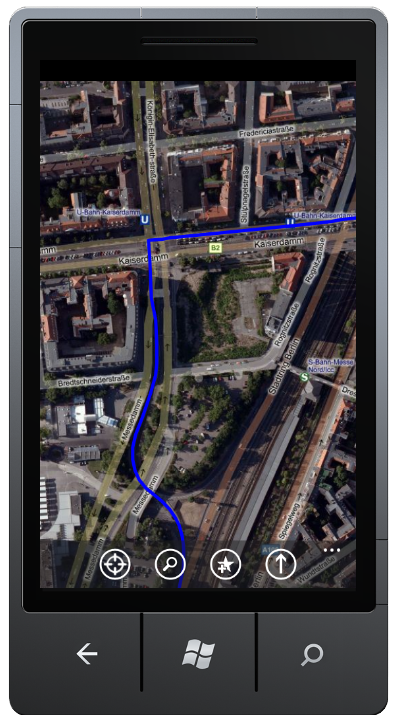
\includegraphics[width=5.0cm,height=10.0cm]{images/route.png}
\end{center}
\caption{Vereinfachte Route}
\end{figure}

\section{Marketplace}
\subsection{Struktur}
\subsection{Entwicklung}
\subsection{Zukunft der Open Street App}
�berlegung ob kostenpflichtig oder nicht. Werbung. Ver�ffentlichung im April 2011. Wirklich.

\section{Ausblick und Fazit}
\subsection{Weiterentwicklung der Plattform}
\subsection{Chancen f�r die Zukunft}
\subsection{Fazit}
Entwickeln toll. Schnelle Ergebnisse.

% Literaturangaben
\begin{thebibliography}{1}
  \bibitem {1} Eine PDF zu Entwicklung
  \bibitem {2} Verweis auf Trainings Projekte und Tutorials von MS
  \bibitem {3} Die APIs (Cloudemade, Yahoo, Bing, Osm)
\end{thebibliography}

\end{document}
